\usetikzlibrary{calc}
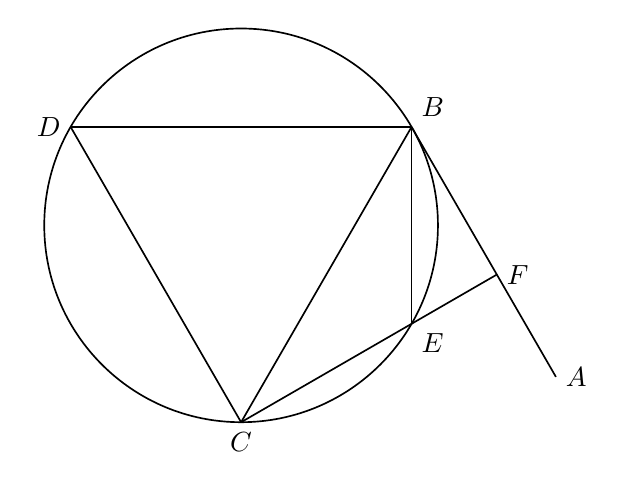
\begin{tikzpicture}[x=1cm,y=1cm,line width=.6pt,font=\normalsize]
\coordinate (O) at (0,0);
\coordinate (D) at (-2.165,1.25);
\coordinate (B) at (2.165,1.25);
\coordinate (C) at (0,-2.5);
\coordinate (E) at (2.165,-1.25);
\coordinate (F) at (3.248,-0.625);
\coordinate (A) at (3.998,-1.924);
\draw (O) circle[radius=2.5cm];
\draw (D)--(B);
\draw (D)--(C);
\draw (B)--(C);
\draw (B)--(E);
\draw (C)--(F);
\draw (B)--(A);
\node[left] at (D) {$D$};
\node[above right] at (B) {$B$};
\node[below] at (C) {$C$};
\node[below right] at (E) {$E$};
\node[right] at (F) {$F$};
\node[right] at (A) {$A$};
\end{tikzpicture}
